% Options for packages loaded elsewhere
\PassOptionsToPackage{unicode}{hyperref}
\PassOptionsToPackage{hyphens}{url}
\PassOptionsToPackage{dvipsnames,svgnames,x11names}{xcolor}
%
\documentclass[
  oneclumn]{article}

\usepackage{amsmath,amssymb}
\usepackage{iftex}
\ifPDFTeX
  \usepackage[T1]{fontenc}
  \usepackage[utf8]{inputenc}
  \usepackage{textcomp} % provide euro and other symbols
\else % if luatex or xetex
  \usepackage{unicode-math}
  \defaultfontfeatures{Scale=MatchLowercase}
  \defaultfontfeatures[\rmfamily]{Ligatures=TeX,Scale=1}
\fi
\usepackage{lmodern}
\ifPDFTeX\else  
    % xetex/luatex font selection
\fi
% Use upquote if available, for straight quotes in verbatim environments
\IfFileExists{upquote.sty}{\usepackage{upquote}}{}
\IfFileExists{microtype.sty}{% use microtype if available
  \usepackage[]{microtype}
  \UseMicrotypeSet[protrusion]{basicmath} % disable protrusion for tt fonts
}{}
\makeatletter
\@ifundefined{KOMAClassName}{% if non-KOMA class
  \IfFileExists{parskip.sty}{%
    \usepackage{parskip}
  }{% else
    \setlength{\parindent}{0pt}
    \setlength{\parskip}{6pt plus 2pt minus 1pt}}
}{% if KOMA class
  \KOMAoptions{parskip=half}}
\makeatother
\usepackage{xcolor}
\usepackage[left=35mm,right=35mm,top=15mm,bottom=20mm,noheadfoot]{geometry}
\setlength{\emergencystretch}{3em} % prevent overfull lines
\setcounter{secnumdepth}{-\maxdimen} % remove section numbering
% Make \paragraph and \subparagraph free-standing
\makeatletter
\ifx\paragraph\undefined\else
  \let\oldparagraph\paragraph
  \renewcommand{\paragraph}{
    \@ifstar
      \xxxParagraphStar
      \xxxParagraphNoStar
  }
  \newcommand{\xxxParagraphStar}[1]{\oldparagraph*{#1}\mbox{}}
  \newcommand{\xxxParagraphNoStar}[1]{\oldparagraph{#1}\mbox{}}
\fi
\ifx\subparagraph\undefined\else
  \let\oldsubparagraph\subparagraph
  \renewcommand{\subparagraph}{
    \@ifstar
      \xxxSubParagraphStar
      \xxxSubParagraphNoStar
  }
  \newcommand{\xxxSubParagraphStar}[1]{\oldsubparagraph*{#1}\mbox{}}
  \newcommand{\xxxSubParagraphNoStar}[1]{\oldsubparagraph{#1}\mbox{}}
\fi
\makeatother


\providecommand{\tightlist}{%
  \setlength{\itemsep}{0pt}\setlength{\parskip}{0pt}}\usepackage{longtable,booktabs,array}
\usepackage{calc} % for calculating minipage widths
% Correct order of tables after \paragraph or \subparagraph
\usepackage{etoolbox}
\makeatletter
\patchcmd\longtable{\par}{\if@noskipsec\mbox{}\fi\par}{}{}
\makeatother
% Allow footnotes in longtable head/foot
\IfFileExists{footnotehyper.sty}{\usepackage{footnotehyper}}{\usepackage{footnote}}
\makesavenoteenv{longtable}
\usepackage{graphicx}
\makeatletter
\def\maxwidth{\ifdim\Gin@nat@width>\linewidth\linewidth\else\Gin@nat@width\fi}
\def\maxheight{\ifdim\Gin@nat@height>\textheight\textheight\else\Gin@nat@height\fi}
\makeatother
% Scale images if necessary, so that they will not overflow the page
% margins by default, and it is still possible to overwrite the defaults
% using explicit options in \includegraphics[width, height, ...]{}
\setkeys{Gin}{width=\maxwidth,height=\maxheight,keepaspectratio}
% Set default figure placement to htbp
\makeatletter
\def\fps@figure{htbp}
\makeatother
% definitions for citeproc citations
\NewDocumentCommand\citeproctext{}{}
\NewDocumentCommand\citeproc{mm}{%
  \begingroup\def\citeproctext{#2}\cite{#1}\endgroup}
\makeatletter
 % allow citations to break across lines
 \let\@cite@ofmt\@firstofone
 % avoid brackets around text for \cite:
 \def\@biblabel#1{}
 \def\@cite#1#2{{#1\if@tempswa , #2\fi}}
\makeatother
\newlength{\cslhangindent}
\setlength{\cslhangindent}{1.5em}
\newlength{\csllabelwidth}
\setlength{\csllabelwidth}{3em}
\newenvironment{CSLReferences}[2] % #1 hanging-indent, #2 entry-spacing
 {\begin{list}{}{%
  \setlength{\itemindent}{0pt}
  \setlength{\leftmargin}{0pt}
  \setlength{\parsep}{0pt}
  % turn on hanging indent if param 1 is 1
  \ifodd #1
   \setlength{\leftmargin}{\cslhangindent}
   \setlength{\itemindent}{-1\cslhangindent}
  \fi
  % set entry spacing
  \setlength{\itemsep}{#2\baselineskip}}}
 {\end{list}}
\usepackage{calc}
\newcommand{\CSLBlock}[1]{\hfill\break\parbox[t]{\linewidth}{\strut\ignorespaces#1\strut}}
\newcommand{\CSLLeftMargin}[1]{\parbox[t]{\csllabelwidth}{\strut#1\strut}}
\newcommand{\CSLRightInline}[1]{\parbox[t]{\linewidth - \csllabelwidth}{\strut#1\strut}}
\newcommand{\CSLIndent}[1]{\hspace{\cslhangindent}#1}

\usepackage{inputenc}
\makeatletter
\@ifpackageloaded{caption}{}{\usepackage{caption}}
\AtBeginDocument{%
\ifdefined\contentsname
  \renewcommand*\contentsname{Table of contents}
\else
  \newcommand\contentsname{Table of contents}
\fi
\ifdefined\listfigurename
  \renewcommand*\listfigurename{List of Figures}
\else
  \newcommand\listfigurename{List of Figures}
\fi
\ifdefined\listtablename
  \renewcommand*\listtablename{List of Tables}
\else
  \newcommand\listtablename{List of Tables}
\fi
\ifdefined\figurename
  \renewcommand*\figurename{Figure}
\else
  \newcommand\figurename{Figure}
\fi
\ifdefined\tablename
  \renewcommand*\tablename{Table}
\else
  \newcommand\tablename{Table}
\fi
}
\@ifpackageloaded{float}{}{\usepackage{float}}
\floatstyle{ruled}
\@ifundefined{c@chapter}{\newfloat{codelisting}{h}{lop}}{\newfloat{codelisting}{h}{lop}[chapter]}
\floatname{codelisting}{Listing}
\newcommand*\listoflistings{\listof{codelisting}{List of Listings}}
\makeatother
\makeatletter
\makeatother
\makeatletter
\@ifpackageloaded{caption}{}{\usepackage{caption}}
\@ifpackageloaded{subcaption}{}{\usepackage{subcaption}}
\makeatother

\ifLuaTeX
  \usepackage{selnolig}  % disable illegal ligatures
\fi
\usepackage{bookmark}

\IfFileExists{xurl.sty}{\usepackage{xurl}}{} % add URL line breaks if available
\urlstyle{same} % disable monospaced font for URLs
\hypersetup{
  colorlinks=true,
  linkcolor={blue},
  filecolor={Maroon},
  citecolor={Blue},
  urlcolor={Blue},
  pdfcreator={LaTeX via pandoc}}


\author{}
\date{}

\begin{document}


\section{Universidade Federal de
Pernambuco}\label{universidade-federal-de-pernambuco}

\vspace{-.4cm}

\section{Centro de Ciências Exatas e da
Natureza}\label{centro-de-ciuxeancias-exatas-e-da-natureza}

\vspace{-.4cm}

\section{Departamento de
Estatística}\label{departamento-de-estatuxedstica}

\vspace{.5cm}

\subsection{TÓPICOS ESPECIAIS EM ESTATÍSTICA
COMPUTACIONAL}\label{tuxf3picos-especiais-em-estatuxedstica-computacional}

\vspace{.2cm}

\subsubsection{TITULO: MLP com e sem Dropout na Classificação de Risco
Cardiovascular: Uma Análise
Comparativa}\label{titulo-mlp-com-e-sem-dropout-na-classificauxe7uxe3o-de-risco-cardiovascular-uma-anuxe1lise-comparativa}

\vspace{.5cm}

\subsection{Martha Liliana Huertas
Madrid}\label{martha-liliana-huertas-madrid}

\vspace{.5cm}

\textbf{Data:} 06 de diciembre de 2025 \vspace{.5cm}

\section{1. Introdução.}\label{introduuxe7uxe3o.}

As doenças cardiovasculares (DCV) são a principal causa de mortalidade
mundial, causando aproximadamente 17,9 milhões de mortes anuais. Na
América Latina, representam 30\% dos óbitos, com tendência crescente
devido ao envelhecimento populacional e fatores de risco como
hipertensão, diabetes e obesidade.A identificação precoce permitiria
intervenções preventivas que salvariam vidas e reduziriam custos. Os
escores tradicionais como Framingham e SCORE, baseados em modelos
lineares, não capturam relações não lineares complexas e apresentam
limitações de generalização por terem sido desenvolvidos em populações
específicas.

As Redes Neurais Multicamadas (MLP) oferecem alternativa promissora ao
modelar interações complexas em dados clínicos. Porém, enfrentam o
desafio do sobreajuste (overfitting), que compromete a generalização. O
Dropout, técnica que desativa aleatoriamente neurônios durante o
treinamento, reduz esse problema melhorando a robustez do modelo. Este
trabalho compara modelos MLP com e sem Dropout na classificação de risco
cardiovascular, fornecendo evidência sobre o papel da regularização na
melhoria da precisão preditiva e capacidade de generalização.

\section{2. Fundamentos Teóricos e
Metodológicos}\label{fundamentos-teuxf3ricos-e-metodoluxf3gicos}

\subsection{2.1. Redes Neuronales
Artificiales}\label{redes-neuronales-artificiales}

As Redes Neurais Artificiais (RNAs) são modelos computacionais
inspirados no funcionamento do cérebro biológico, especificamente na
forma como os neurônios processam e transmitem informações. Assim como o
cérebro humano é composto por bilhões de neurônios interconectados, as
RNAs consistem em unidades de processamento simples (neurônio
artificial) organizadas em camadas.(Ferreira 2025c)

\subsubsection{2.1.1. Arquitectura MLP
Implementada}\label{arquitectura-mlp-implementada}

\textbf{Função de ativação ReLU:} \[f(x) = max(0, x)\]

\textbf{Função de ativação Sigmoid:} \[f(x) = \frac{1}{1 + e^{-x}}\]

\subsection{2.2. Técnicas de
Regularização}\label{tuxe9cnicas-de-regularizauxe7uxe3o}

\subsubsection{2.2.1. Dropout}\label{dropout}

O Dropout é uma técnica de regularização que previne o sobreajuste
(overfitting) ao desativar neurônios aleatoriamente durante o
treinamento (Ferreira 2025b).

\subsubsection{2.2.2. Função de Perda}\label{funuxe7uxe3o-de-perda}

\textbf{Entropia Cruzada Binária (Binary Cross-Entropy):}
\[\mathcal{L} = -\frac{1}{N} \sum_{i=1}^{N} [y_i \log(\hat{y}_i) + (1-y_i) \log(1-\hat{y}_i)]\]
Essa função é amplamente utilizada em problemas de classificação
binária, pois mede a diferença entre as probabilidades previstas pelo
modelo.

\subsection{2.3. Otimização com Adam}\label{otimizauxe7uxe3o-com-adam}

Algoritmo que adapta a learning rate por parâmetro:

\[m_t = \beta_1 m_{t-1} + (1-\beta_1)g_t\]
\[v_t = \beta_2 v_{t-1} + (1-\beta_2)g_t^2\]
\[\theta_t = \theta_{t-1} - \alpha\frac{\hat{m}_t}{\sqrt{\hat{v}_t} + \epsilon}\]

\subsection{2.4. Métricas de
Avaliação}\label{muxe9tricas-de-avaliauxe7uxe3o}

\subsubsection{2.4.1.Matriz de Confusão}\label{matriz-de-confusuxe3o}

A matriz de confusão é uma ferramenta utilizada para avaliar o
desempenho de modelos de classificação. Ela organiza os resultados
previstos pelo modelo em comparação com os valores reais, permitindo
identificar acertos e erros em cada classe.

\[
\begin{array}{c|cc}
 & \text{Predição 0} & \text{Predição 1} \\
\hline
\text{Real 0} & TN & FP \\
\text{Real 1} & FN & TP \\
\end{array}
\]

\subsubsection{2.4.2. Métricas Principais}\label{muxe9tricas-principais}

\begin{itemize}
\item
  Accuracy: \(\frac{VP + VN}{Total}\)
\item
  Precision: \(\frac{VP}{VP + FP}\)
\item
  Recall: \(\frac{VP}{VP + FN}\)
\item
  F1-Score:
  \(2\times\frac{Precision \times Recall}{Precision + Recall}\)
\end{itemize}

\subsubsection{2.4.3. Curva ROC y AUC}\label{curva-roc-y-auc}

A curva ROC mostra o trade-off entre a Taxa de Verdadeiros Positivos
(TPR) e a Taxa de Falsos Positivos (FPR):

\[TPR = \frac{TP}{TP + FN}\] \[FPR = \frac{FP}{FP + TN}\]

O AUC (Area Under Curve) quantifica a capacidade discriminativa do
modelo em todos os limiares (thresholds). {[}Ferreira (2025a)

\section{3. Aplicação}\label{aplicauxe7uxe3o}

\subsection{3.1. Descrição do Dataset e Análise
Exploratória}\label{descriuxe7uxe3o-do-dataset-e-anuxe1lise-exploratuxf3ria}

Foi utilizada a base de dados Cardiovascular Disease, que contém 70.000
registros de pacientes com 12 variáveis clínicas coletadas por meio de
exames médicos.

\begin{longtable}[]{@{}ccc@{}}
\caption{Distribuição de
pacientes}\label{tbl-distribucion}\tabularnewline
\toprule\noalign{}
\textbf{Grupo de pacientes} & \textbf{n} & \textbf{\%} \\
\midrule\noalign{}
\endfirsthead
\toprule\noalign{}
\textbf{Grupo de pacientes} & \textbf{n} & \textbf{\%} \\
\midrule\noalign{}
\endhead
\bottomrule\noalign{}
\endlastfoot
\textbf{Pacientes saudáveis} & 35.021 & 50.03\% \\
\textbf{Pacientes com doença cardiovascular} & 34.979 & 49.97\% \\
\textbf{Total} & \textbf{70,000} & \textbf{100\%} \\
\end{longtable}

\begin{center}
\footnotesize \textit{Fonte: Elaboração própria}
\end{center}

A Table~\ref{tbl-distribucion} detalha a composição do conjunto de
dados, revelando uma distribuição balanceada das classes-alvo: 49,97\%
corresponde a pacientes com diagnóstico positivo de doença
cardiovascular, enquanto os 50,03\% restantes representam pacientes sem
a patologia.

\textbf{Variáveis do Dataset:}

-Demográficas: idade, gênero, altura, peso, BMI (Masa corporal)

-Sinais vitais: pressão arterial sistólica e diastólica

-Fatores de risco: Colesterol (1: normal, 2: alto, 3: muito alto),
Glicose (1: normal, 2: alto, 3: muito alto)

-Hábitos: tabagismo, consumo de álcool, atividade física

-Variável alvo: presença de doença cardiovascular (1: sim, 0: não)

\textbf{Estatísticas Descritivas:}

\begin{longtable}[]{@{}
  >{\centering\arraybackslash}p{(\columnwidth - 8\tabcolsep) * \real{0.2603}}
  >{\centering\arraybackslash}p{(\columnwidth - 8\tabcolsep) * \real{0.1507}}
  >{\centering\arraybackslash}p{(\columnwidth - 8\tabcolsep) * \real{0.2603}}
  >{\centering\arraybackslash}p{(\columnwidth - 8\tabcolsep) * \real{0.1644}}
  >{\centering\arraybackslash}p{(\columnwidth - 8\tabcolsep) * \real{0.1644}}@{}}
\caption{Estatística Descriptivas}\label{tbl-est}\tabularnewline
\toprule\noalign{}
\begin{minipage}[b]{\linewidth}\centering
\textbf{Variável}
\end{minipage} & \begin{minipage}[b]{\linewidth}\centering
\textbf{Média}
\end{minipage} & \begin{minipage}[b]{\linewidth}\centering
\textbf{Desvio Padrão}
\end{minipage} & \begin{minipage}[b]{\linewidth}\centering
\textbf{Mínimo}
\end{minipage} & \begin{minipage}[b]{\linewidth}\centering
\textbf{Máximo}
\end{minipage} \\
\midrule\noalign{}
\endfirsthead
\toprule\noalign{}
\begin{minipage}[b]{\linewidth}\centering
\textbf{Variável}
\end{minipage} & \begin{minipage}[b]{\linewidth}\centering
\textbf{Média}
\end{minipage} & \begin{minipage}[b]{\linewidth}\centering
\textbf{Desvio Padrão}
\end{minipage} & \begin{minipage}[b]{\linewidth}\centering
\textbf{Mínimo}
\end{minipage} & \begin{minipage}[b]{\linewidth}\centering
\textbf{Máximo}
\end{minipage} \\
\midrule\noalign{}
\endhead
\bottomrule\noalign{}
\endlastfoot
\textbf{Idade (anos)} & 53.3 & 6.8 & 39 & 65 \\
\textbf{IMC (kg/m²)} & 27.6 & 4.8 & 15.2 & 49.8 \\
\textbf{P.Sistólica} & 128.6 & 18.2 & 90 & 180 \\
\textbf{P. Diastólica} & 96.6 & 11.8 & 60 & 120 \\
\textbf{Altura (cm)} & 164.4 & 8.2 & 145 & 185 \\
\textbf{Peso (kg)} & 74.2 & 14.1 & 41 & 120 \\
\end{longtable}

\begin{center}
\footnotesize \textit{Fonte: Elaboração própria}
\end{center}

Na Table~\ref{tbl-est} a população apresentou uma idade média de 53,3
anos (DP: 6,8) e um IMC de 27,6 kg/m² (DP: 4,8), situando-se na faixa de
meia-idade com predominância de sobrepeso. As medições de pressão
arterial mostraram valores médios de 128,6/96,6 mmHg, dentro dos
intervalos de pré-hipertensão.

\section{3.2 Pré-processamento de
Dados}\label{pruxe9-processamento-de-dados}

Uma vez concluída a análise exploratória, os dados foram preparados para
o modelamento preditivo, selecionando doze variáveis como preditores:
idade, gênero, altura, peso, IMC, pressão arterial sistólica e
diastólica, níveis de colesterol e glicose, tabagismo, consumo de álcool
e atividade física. A variável alvo foi o diagnóstico de doença
cardiovascular, definindo um problema de classificação binária. Para o
pré-processamento, as variáveis categóricas (colesterol e glicose) foram
transformadas por meio de codificação one-hot, expandindo o conjunto
para catorze variáveis preditoras. Os dados foram divididos em 70\% para
treinamento e 30\% para teste com amostragem estratificada, e todas as
variáveis numéricas foram padronizadas.

\section{3.3 Arquitetura do Modelo}\label{arquitetura-do-modelo}

Foi projetada uma rede neural multicamada com catorze entradas e três
camadas ocultas em progressão decrescente: 128, 64 e 32 neurônios
respectivamente, utilizando a função de ativação ReLU. Essa arquitetura
progressiva permite ao modelo aprender representações hierárquicas dos
dados, capturando relações complexas entre variáveis sem gerar
sobreajuste. A camada de saída conta com um neurônio e ativação
sigmoide, gerando probabilidades interpretáveis de risco cardiovascular
no intervalo {[}0,1{]}.

Foram desenvolvidas duas versões do modelo com arquitetura idêntica: uma
incorporando dropout com taxas progressivas (40\%, 30\%, 20\%) nas
camadas ocultas, e outra sem qualquer regularização.

Ambos os modelos foram treinados com entropia cruzada binária como
função de perda, otimizador Adam com taxa de aprendizado de 0,001, 50
épocas de treinamento, tamanho de lote de 128 amostras e 20\% do
conjunto de treinamento reservado para validação. O desempenho foi
avaliado por meio das métricas de exatidão (accuracy) e área sob a curva
ROC (AUC). A Table~\ref{tbl-comp} apresenta as métricas de classificação
obtidas no conjunto de teste para ambas as arquiteturas.

\begin{longtable}[]{@{}ccc@{}}
\caption{Comparação dos Modelos}\label{tbl-comp}\tabularnewline
\toprule\noalign{}
\textbf{Métricas} & \textbf{MLP com Dropout} & \textbf{MLP sem
Dropout} \\
\midrule\noalign{}
\endfirsthead
\toprule\noalign{}
\textbf{Métricas} & \textbf{MLP com Dropout} & \textbf{MLP sem
Dropout} \\
\midrule\noalign{}
\endhead
\bottomrule\noalign{}
\endlastfoot
AUC & 0.7984 & 0.7828 \\
Accuracy & 0.7326 & 0.7222 \\
Precisão & 0.7514 & 0.7405 \\
Recall & 0.6859 & 0.6740 \\
F1-Score & 0.7172 & 0.7057 \\
\end{longtable}

\begin{center}
\footnotesize \textit{Fonte: Elaboração própria}
\end{center}

A Table~\ref{tbl-comp} mostra que o modelo com dropout superou o modelo
sem regularização em todas as métricas. O modelo regularizado alcançou
um AUC de 0,7984 comparado com 0,7828, uma acurácia de 73,26\% frente a
72,22\%, precisão de 75,14\% comparado com 74,05\%, recall de 68,59\%
frente a 67,40\% e F1-Score de 71,72\% frente a 70,57\%. Esses
resultados demonstram que o dropout melhora a capacidade preditiva do
modelo.

\begin{figure}

\centering{

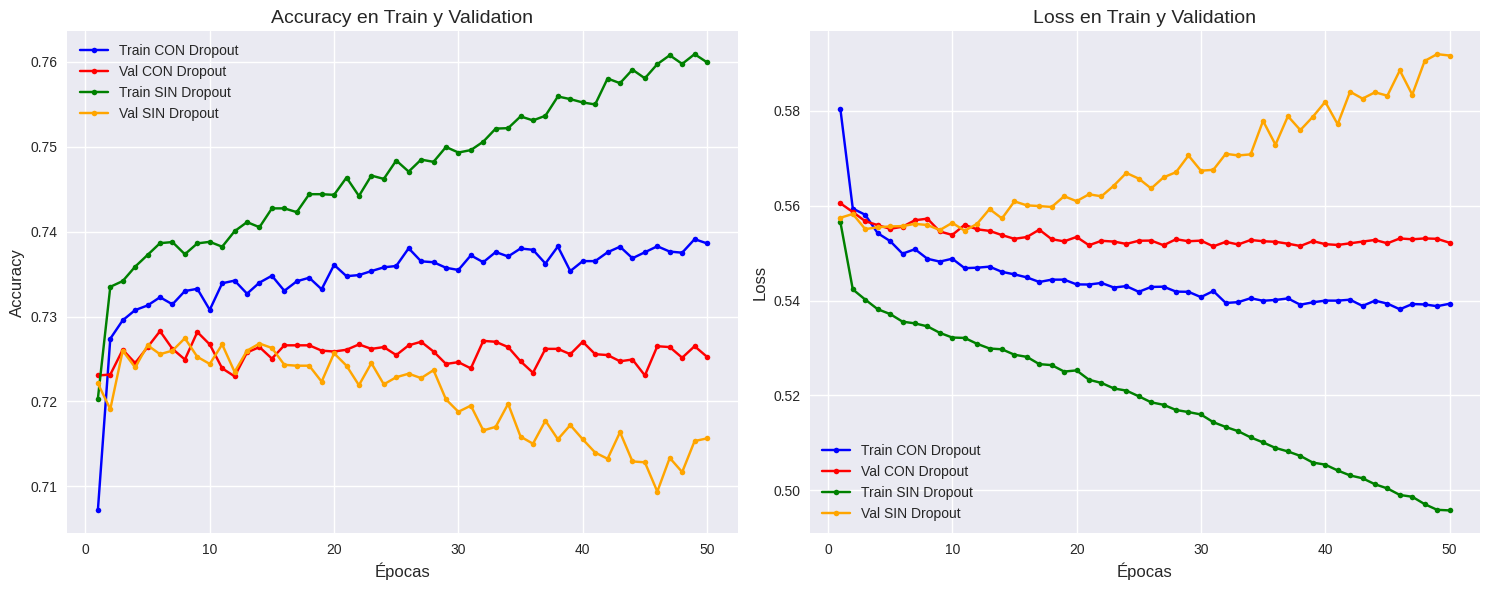
\includegraphics[width=1\textwidth,height=\textheight]{Loss y acuracia.png}

}

\caption{\label{fig-conysim}Avaliação de Overfitting: Comparação de
Modelos com/sem Dropout}

\end{figure}%

\begin{minipage}{\textwidth}
\centering
\vspace{-10pt}
\footnotesize \textit{Fonte: Elaboração própria}
\end{minipage}

A Figure~\ref{fig-conysim} confirma a superioridade do modelo
regularizado através das curvas de aprendizagem. O modelo sem dropout
apresenta overfitting evidente, com divergência acentuada entre treino e
validação, indicando memorização sem generalização adequada. Já o modelo
com dropout exibe curvas mais próximas e paralelas, com perda de
validação decrescente e estável, demonstrando aprendizado de padrões
generalizáveis. A suavidade das trajetórias contrasta com as flutuações
do modelo não regularizado, evidenciando maior estabilidade na
otimização.

Esta capacidade de generalização se reflete de maneira significativa na
métrica de discriminação do modelo, um dos indicadores mais importantes
para avaliar o desempenho preditivo em problemas de classificação
binária. A área sob a curva ROC (AUC), cujos valores numéricos são
apresentados na Table~\ref{tbl-comp}, é visualizada graficamente na
Figure~\ref{fig-curvaor}, que permite uma comparação detalhada do
desempenho discriminativo de ambos os modelos ao longo de diferentes
limiares de classificação.

A análise da curva apresentada na Figure~\ref{fig-curvaor} revela que o
modelo com dropout mantém uma taxa de verdadeiros positivos
consistentemente superior em toda a faixa de taxas de falsos positivos,
desde os valores mais baixos até os mais elevados. Este comportamento
uniforme ao longo de todo o espectro de limiares confirma sua melhor
capacidade de distinguir entre pacientes com e sem risco cardiovascular,
independentemente do ponto de corte escolhido para a tomada de decisão
clínica. A diferença observada de 0,014 pontos na AUC, embora possa
parecer numericamente modesta à primeira vista, representa na verdade
uma melhoria relevante e clinicamente significativa no contexto da
predição de risco cardiovascular. Em ambientes clínicos reais, onde
decisões sobre intervenções preventivas, prescrição de medicamentos ou
encaminhamento para procedimentos especializados dependem crucialmente
da precisão das estimativas de risco, cada ponto percentual adicional na
capacidade de discriminação pode ter impactos substanciais nas decisões
médicas e, consequentemente, nos desfechos de saúde dos pacientes. Esta
melhoria na discriminação traduz-se em uma capacidade aprimorada de
identificar corretamente os pacientes que realmente necessitam de
intervenção, ao mesmo tempo que reduz falsos alarmes que poderiam
resultar em tratamentos desnecessários e custos evitáveis ao sistema de
saúde.

Além da capacidade discriminativa avaliada pelas curvas ROC, é crucial
examinar a qualidadedas probabilidades geradas pelo modelo. Em
aplicações clínicas, não basta que o modelo dis-tinga bem entre classes;
as probabilidades preditas devem refletir com precisão o risco real
dospacientes. A calibração adequada é fundamental para que os
profissionais de saúde possam tomar decisões terapêuticas confiáveis,
baseando-se nas estimativas de risco fornecidas.

\begin{figure}

\centering{

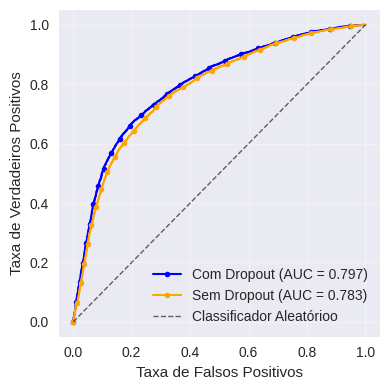
\includegraphics{Curvaor.png}

}

\caption{\label{fig-curvaor}Comparação das Curvas ROC: Modelo com
Dropout vs.~Sem Dropout}

\end{figure}%

\begin{minipage}{\textwidth}
\centering
\vspace{-10pt}
\footnotesize \textit{Fonte: Elaboração própria}
\end{minipage}

\begin{figure}

\centering{

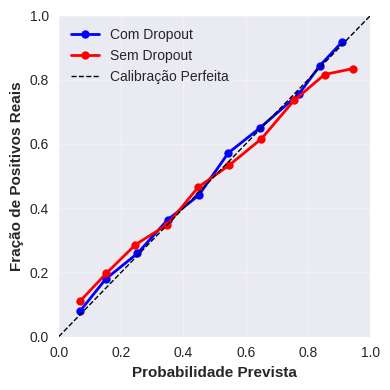
\includegraphics{calibracion.png}

}

\caption{\label{fig-calibracion}Análise de Calibração: Confiabilidade
das Probabilidades Preditas}

\end{figure}%

\begin{minipage}{\textwidth}
\centering
\vspace{-10pt}
\footnotesize \textit{Fonte: Elaboração própria}
\end{minipage}

A Figure~\ref{fig-calibracion} mostra que o modelo com dropout está mais
alinhado com a linha de calibração perfeita, indicando que suas
probabilidades previstas refletem com maior precisão a proporção real de
resultados positivos.

\section{4. Conclusão}\label{conclusuxe3o}

Este estudo demonstrou a eficácia do dropout como técnica de
regularização em redes neurais multicamadas para classificação de risco
cardiovascular. O modelo regularizado superou o modelo base em todas as
métricas As curvas de aprendizagem confirmaram que o dropout controla
eficazmente o overfitting, mantendo convergência estável entre treino e
validação. Adicionalmente, a análise de calibração revelou que o modelo
regularizado gera probabilidades mais confiáveis, aspecto crucial para
aplicações clínicas onde as predições impactam decisões médicas. Os
resultados evidenciam que a regularização via dropout é essencial para
desenvolver modelos preditivos robustos em saúde, equilibrando
adequadamente complexidade e capacidade de generalização.

\section{5. Referencias
Bibliograficas}\label{referencias-bibliograficas}

\phantomsection\label{refs}
\begin{CSLReferences}{1}{0}
\bibitem[\citeproctext]{ref-teec2024assessing}
Ferreira, Jodavid. 2025a. {``Avaliando a Acurácia Do Modelo.''} Aula 13
- TEEC.
\url{https://jodavid.github.io/computationalstatisticstopics/TEEC/13_assessing_model_accuracy/assessing_model_accuracy.html}.

\bibitem[\citeproctext]{ref-teec2024dropout}
---------. 2025b. {``Dropout Em Redes Neurais.''} Aula 19 - TEEC.
\url{https://jodavid.github.io/computationalstatisticstopics/TEEC/19_Dropout/dropout.html}.

\bibitem[\citeproctext]{ref-teec2024neuralintro}
---------. 2025c. {``Redes Neurais Artificiais e MLP.''} Aula 15 - TEEC.
\url{https://jodavid.github.io/computationalstatisticstopics/TEEC/15_RedesNeurais_e_MLP/Cerebro_e_Redes_Neurais.html}.

\end{CSLReferences}




\end{document}
